% Options for packages loaded elsewhere
\PassOptionsToPackage{unicode}{hyperref}
\PassOptionsToPackage{hyphens}{url}
%
\documentclass[
]{article}
\usepackage{amsmath,amssymb}
\usepackage{lmodern}
\usepackage{iftex}
\ifPDFTeX
  \usepackage[T1]{fontenc}
  \usepackage[utf8]{inputenc}
  \usepackage{textcomp} % provide euro and other symbols
\else % if luatex or xetex
  \usepackage{unicode-math}
  \defaultfontfeatures{Scale=MatchLowercase}
  \defaultfontfeatures[\rmfamily]{Ligatures=TeX,Scale=1}
\fi
% Use upquote if available, for straight quotes in verbatim environments
\IfFileExists{upquote.sty}{\usepackage{upquote}}{}
\IfFileExists{microtype.sty}{% use microtype if available
  \usepackage[]{microtype}
  \UseMicrotypeSet[protrusion]{basicmath} % disable protrusion for tt fonts
}{}
\makeatletter
\@ifundefined{KOMAClassName}{% if non-KOMA class
  \IfFileExists{parskip.sty}{%
    \usepackage{parskip}
  }{% else
    \setlength{\parindent}{0pt}
    \setlength{\parskip}{6pt plus 2pt minus 1pt}}
}{% if KOMA class
  \KOMAoptions{parskip=half}}
\makeatother
\usepackage{xcolor}
\usepackage[margin=1in]{geometry}
\usepackage{color}
\usepackage{fancyvrb}
\newcommand{\VerbBar}{|}
\newcommand{\VERB}{\Verb[commandchars=\\\{\}]}
\DefineVerbatimEnvironment{Highlighting}{Verbatim}{commandchars=\\\{\}}
% Add ',fontsize=\small' for more characters per line
\usepackage{framed}
\definecolor{shadecolor}{RGB}{248,248,248}
\newenvironment{Shaded}{\begin{snugshade}}{\end{snugshade}}
\newcommand{\AlertTok}[1]{\textcolor[rgb]{0.94,0.16,0.16}{#1}}
\newcommand{\AnnotationTok}[1]{\textcolor[rgb]{0.56,0.35,0.01}{\textbf{\textit{#1}}}}
\newcommand{\AttributeTok}[1]{\textcolor[rgb]{0.77,0.63,0.00}{#1}}
\newcommand{\BaseNTok}[1]{\textcolor[rgb]{0.00,0.00,0.81}{#1}}
\newcommand{\BuiltInTok}[1]{#1}
\newcommand{\CharTok}[1]{\textcolor[rgb]{0.31,0.60,0.02}{#1}}
\newcommand{\CommentTok}[1]{\textcolor[rgb]{0.56,0.35,0.01}{\textit{#1}}}
\newcommand{\CommentVarTok}[1]{\textcolor[rgb]{0.56,0.35,0.01}{\textbf{\textit{#1}}}}
\newcommand{\ConstantTok}[1]{\textcolor[rgb]{0.00,0.00,0.00}{#1}}
\newcommand{\ControlFlowTok}[1]{\textcolor[rgb]{0.13,0.29,0.53}{\textbf{#1}}}
\newcommand{\DataTypeTok}[1]{\textcolor[rgb]{0.13,0.29,0.53}{#1}}
\newcommand{\DecValTok}[1]{\textcolor[rgb]{0.00,0.00,0.81}{#1}}
\newcommand{\DocumentationTok}[1]{\textcolor[rgb]{0.56,0.35,0.01}{\textbf{\textit{#1}}}}
\newcommand{\ErrorTok}[1]{\textcolor[rgb]{0.64,0.00,0.00}{\textbf{#1}}}
\newcommand{\ExtensionTok}[1]{#1}
\newcommand{\FloatTok}[1]{\textcolor[rgb]{0.00,0.00,0.81}{#1}}
\newcommand{\FunctionTok}[1]{\textcolor[rgb]{0.00,0.00,0.00}{#1}}
\newcommand{\ImportTok}[1]{#1}
\newcommand{\InformationTok}[1]{\textcolor[rgb]{0.56,0.35,0.01}{\textbf{\textit{#1}}}}
\newcommand{\KeywordTok}[1]{\textcolor[rgb]{0.13,0.29,0.53}{\textbf{#1}}}
\newcommand{\NormalTok}[1]{#1}
\newcommand{\OperatorTok}[1]{\textcolor[rgb]{0.81,0.36,0.00}{\textbf{#1}}}
\newcommand{\OtherTok}[1]{\textcolor[rgb]{0.56,0.35,0.01}{#1}}
\newcommand{\PreprocessorTok}[1]{\textcolor[rgb]{0.56,0.35,0.01}{\textit{#1}}}
\newcommand{\RegionMarkerTok}[1]{#1}
\newcommand{\SpecialCharTok}[1]{\textcolor[rgb]{0.00,0.00,0.00}{#1}}
\newcommand{\SpecialStringTok}[1]{\textcolor[rgb]{0.31,0.60,0.02}{#1}}
\newcommand{\StringTok}[1]{\textcolor[rgb]{0.31,0.60,0.02}{#1}}
\newcommand{\VariableTok}[1]{\textcolor[rgb]{0.00,0.00,0.00}{#1}}
\newcommand{\VerbatimStringTok}[1]{\textcolor[rgb]{0.31,0.60,0.02}{#1}}
\newcommand{\WarningTok}[1]{\textcolor[rgb]{0.56,0.35,0.01}{\textbf{\textit{#1}}}}
\usepackage{graphicx}
\makeatletter
\def\maxwidth{\ifdim\Gin@nat@width>\linewidth\linewidth\else\Gin@nat@width\fi}
\def\maxheight{\ifdim\Gin@nat@height>\textheight\textheight\else\Gin@nat@height\fi}
\makeatother
% Scale images if necessary, so that they will not overflow the page
% margins by default, and it is still possible to overwrite the defaults
% using explicit options in \includegraphics[width, height, ...]{}
\setkeys{Gin}{width=\maxwidth,height=\maxheight,keepaspectratio}
% Set default figure placement to htbp
\makeatletter
\def\fps@figure{htbp}
\makeatother
\setlength{\emergencystretch}{3em} % prevent overfull lines
\providecommand{\tightlist}{%
  \setlength{\itemsep}{0pt}\setlength{\parskip}{0pt}}
\setcounter{secnumdepth}{-\maxdimen} % remove section numbering
\ifLuaTeX
  \usepackage{selnolig}  % disable illegal ligatures
\fi
\IfFileExists{bookmark.sty}{\usepackage{bookmark}}{\usepackage{hyperref}}
\IfFileExists{xurl.sty}{\usepackage{xurl}}{} % add URL line breaks if available
\urlstyle{same} % disable monospaced font for URLs
\hypersetup{
  pdftitle={pstat131-hw2},
  pdfauthor={Sissi Shen},
  hidelinks,
  pdfcreator={LaTeX via pandoc}}

\title{pstat131-hw2}
\author{Sissi Shen}
\date{2022-10-15}

\begin{document}
\maketitle

\begin{Shaded}
\begin{Highlighting}[]
\NormalTok{abalone }\OtherTok{=} \FunctionTok{read.csv}\NormalTok{(}\AttributeTok{file=}\StringTok{\textquotesingle{}abalone.csv\textquotesingle{}}\NormalTok{)}
\end{Highlighting}
\end{Shaded}

Question 1:\n

\begin{Shaded}
\begin{Highlighting}[]
\FunctionTok{library}\NormalTok{(dplyr)}
\end{Highlighting}
\end{Shaded}

\begin{verbatim}
## 
## Attaching package: 'dplyr'
\end{verbatim}

\begin{verbatim}
## The following objects are masked from 'package:stats':
## 
##     filter, lag
\end{verbatim}

\begin{verbatim}
## The following objects are masked from 'package:base':
## 
##     intersect, setdiff, setequal, union
\end{verbatim}

\begin{Shaded}
\begin{Highlighting}[]
\FunctionTok{library}\NormalTok{(tidymodels)}
\end{Highlighting}
\end{Shaded}

\begin{verbatim}
## -- Attaching packages -------------------------------------- tidymodels 1.0.0 --
\end{verbatim}

\begin{verbatim}
## v broom        1.0.1     v rsample      1.1.0
## v dials        1.0.0     v tibble       3.1.8
## v ggplot2      3.3.6     v tidyr        1.2.0
## v infer        1.0.3     v tune         1.0.0
## v modeldata    1.0.1     v workflows    1.0.0
## v parsnip      1.0.1     v workflowsets 1.0.0
## v purrr        0.3.4     v yardstick    1.1.0
## v recipes      1.0.1
\end{verbatim}

\begin{verbatim}
## -- Conflicts ----------------------------------------- tidymodels_conflicts() --
## x purrr::discard() masks scales::discard()
## x dplyr::filter()  masks stats::filter()
## x dplyr::lag()     masks stats::lag()
## x recipes::step()  masks stats::step()
## * Dig deeper into tidy modeling with R at https://www.tmwr.org
\end{verbatim}

\begin{Shaded}
\begin{Highlighting}[]
\FunctionTok{library}\NormalTok{(tidyverse)}
\end{Highlighting}
\end{Shaded}

\begin{verbatim}
## -- Attaching packages --------------------------------------- tidyverse 1.3.2 --
\end{verbatim}

\begin{verbatim}
## v readr   2.1.2     v forcats 0.5.1
## v stringr 1.4.0     
## -- Conflicts ------------------------------------------ tidyverse_conflicts() --
## x readr::col_factor() masks scales::col_factor()
## x purrr::discard()    masks scales::discard()
## x dplyr::filter()     masks stats::filter()
## x stringr::fixed()    masks recipes::fixed()
## x dplyr::lag()        masks stats::lag()
## x readr::spec()       masks yardstick::spec()
\end{verbatim}

\begin{Shaded}
\begin{Highlighting}[]
\NormalTok{abalone }\OtherTok{\textless{}{-}}\NormalTok{ abalone }\SpecialCharTok{\%\textgreater{}\%}
  \FunctionTok{mutate}\NormalTok{(}\AttributeTok{age =}\NormalTok{ rings }\SpecialCharTok{+} \FloatTok{1.5}\NormalTok{)}
\FunctionTok{hist}\NormalTok{(abalone}\SpecialCharTok{$}\NormalTok{age)}
\end{Highlighting}
\end{Shaded}

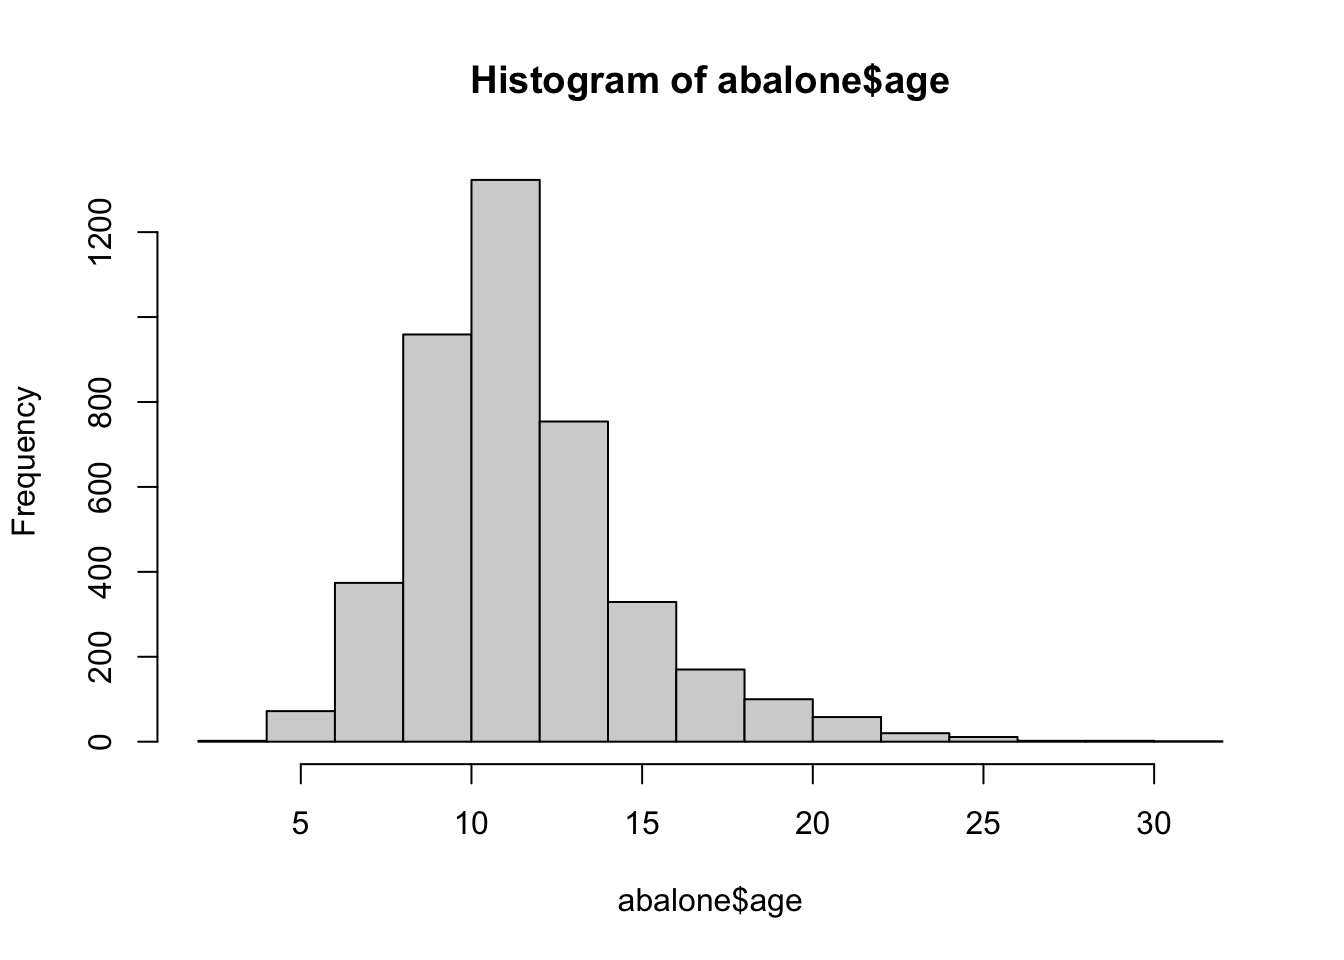
\includegraphics{pstat122-hw2_files/figure-latex/unnamed-chunk-2-1.pdf}
\n From the histogram, we can tell that the distribution of abalone's
age is skewed to the left, which indicates that most abalone in our data
sample are relatively young. \n

Question 2:

\begin{Shaded}
\begin{Highlighting}[]
\FunctionTok{set.seed}\NormalTok{(}\DecValTok{1029}\NormalTok{)}
\NormalTok{abalone\_split }\OtherTok{\textless{}{-}} \FunctionTok{initial\_split}\NormalTok{(abalone, }\AttributeTok{prop=}\FloatTok{0.8}\NormalTok{, }\AttributeTok{strata =}\NormalTok{ age)}
\NormalTok{abalone\_train }\OtherTok{\textless{}{-}} \FunctionTok{training}\NormalTok{(abalone\_split)}
\NormalTok{abalone\_test }\OtherTok{\textless{}{-}} \FunctionTok{testing}\NormalTok{(abalone\_split)}
\end{Highlighting}
\end{Shaded}

\n

Question 3:

\begin{Shaded}
\begin{Highlighting}[]
\NormalTok{abalone\_train }\OtherTok{\textless{}{-}}\NormalTok{ abalone\_train }\SpecialCharTok{\%\textgreater{}\%} \FunctionTok{select}\NormalTok{(}\SpecialCharTok{{-}}\NormalTok{rings)}
\NormalTok{abalone\_test }\OtherTok{\textless{}{-}}\NormalTok{ abalone\_test }\SpecialCharTok{\%\textgreater{}\%} \FunctionTok{select}\NormalTok{(}\SpecialCharTok{{-}}\NormalTok{rings)}
\end{Highlighting}
\end{Shaded}

\n

We should not include the variable ``rings'' because it is basically the
outcome ``age'' that we want to predict. \n

\begin{Shaded}
\begin{Highlighting}[]
\NormalTok{simple\_abalone\_recipe }\OtherTok{\textless{}{-}} \FunctionTok{recipe}\NormalTok{(age }\SpecialCharTok{\textasciitilde{}}\NormalTok{ ., }\AttributeTok{data =}\NormalTok{ abalone\_train)}
\NormalTok{simple\_abalone\_recipe}
\end{Highlighting}
\end{Shaded}

\begin{verbatim}
## Recipe
## 
## Inputs:
## 
##       role #variables
##    outcome          1
##  predictor          8
\end{verbatim}

\begin{Shaded}
\begin{Highlighting}[]
\NormalTok{abalone\_recipe }\OtherTok{\textless{}{-}} \FunctionTok{recipe}\NormalTok{(age }\SpecialCharTok{\textasciitilde{}}\NormalTok{ ., }\AttributeTok{data =}\NormalTok{ abalone\_train) }\SpecialCharTok{\%\textgreater{}\%}
  \FunctionTok{step\_dummy}\NormalTok{(}\FunctionTok{all\_nominal\_predictors}\NormalTok{()) }\SpecialCharTok{\%\textgreater{}\%}
  \FunctionTok{step\_interact}\NormalTok{(}\AttributeTok{terms =} \SpecialCharTok{\textasciitilde{}} \FunctionTok{starts\_with}\NormalTok{(}\StringTok{"type"}\NormalTok{)}\SpecialCharTok{:}\NormalTok{shucked\_weight) }\SpecialCharTok{\%\textgreater{}\%}
  \FunctionTok{step\_interact}\NormalTok{(}\AttributeTok{terms =} \SpecialCharTok{\textasciitilde{}}\NormalTok{ longest\_shell}\SpecialCharTok{:}\NormalTok{diameter) }\SpecialCharTok{\%\textgreater{}\%}
  \FunctionTok{step\_interact}\NormalTok{(}\AttributeTok{terms =} \SpecialCharTok{\textasciitilde{}}\NormalTok{ shucked\_weight}\SpecialCharTok{:}\NormalTok{shell\_weight) }\SpecialCharTok{\%\textgreater{}\%}
  \FunctionTok{step\_center}\NormalTok{(}\FunctionTok{all\_numeric\_predictors}\NormalTok{()) }\SpecialCharTok{\%\textgreater{}\%}
  \FunctionTok{step\_scale}\NormalTok{(}\FunctionTok{all\_numeric\_predictors}\NormalTok{())}
\end{Highlighting}
\end{Shaded}

\n

Question 4:

\begin{Shaded}
\begin{Highlighting}[]
\NormalTok{lm\_model }\OtherTok{\textless{}{-}} \FunctionTok{linear\_reg}\NormalTok{() }\SpecialCharTok{\%\textgreater{}\%}
  \FunctionTok{set\_engine}\NormalTok{(}\StringTok{"lm"}\NormalTok{)}
\end{Highlighting}
\end{Shaded}

\n

Question 5:

\begin{Shaded}
\begin{Highlighting}[]
\NormalTok{lm\_wflow }\OtherTok{\textless{}{-}} \FunctionTok{workflow}\NormalTok{() }\SpecialCharTok{\%\textgreater{}\%} 
  \FunctionTok{add\_model}\NormalTok{(lm\_model) }\SpecialCharTok{\%\textgreater{}\%} 
  \FunctionTok{add\_recipe}\NormalTok{(abalone\_recipe)}
\end{Highlighting}
\end{Shaded}

\n

Question 6:

\begin{Shaded}
\begin{Highlighting}[]
\NormalTok{lm\_fit }\OtherTok{\textless{}{-}} \FunctionTok{fit}\NormalTok{(lm\_wflow, abalone\_train)}
\NormalTok{lm\_fit }\SpecialCharTok{\%\textgreater{}\%}
  \FunctionTok{extract\_fit\_parsnip}\NormalTok{()}\SpecialCharTok{\%\textgreater{}\%}
  \FunctionTok{tidy}\NormalTok{()}
\end{Highlighting}
\end{Shaded}

\begin{verbatim}
## # A tibble: 14 x 5
##    term                          estimate std.error statistic  p.value
##    <chr>                            <dbl>     <dbl>     <dbl>    <dbl>
##  1 (Intercept)                     11.4      0.0371    308.   0       
##  2 longest_shell                    0.747    0.281       2.66 7.86e- 3
##  3 diameter                         2.07     0.306       6.75 1.74e-11
##  4 height                           0.226    0.0697      3.24 1.19e- 3
##  5 whole_weight                     5.41     0.414      13.1  3.25e-38
##  6 shucked_weight                  -4.31     0.253     -17.0  1.67e-62
##  7 viscera_weight                  -0.976    0.161      -6.07 1.42e- 9
##  8 shell_weight                     1.58     0.214       7.38 2.00e-13
##  9 type_I                          -1.06     0.114      -9.26 3.72e-20
## 10 type_M                          -0.345    0.102      -3.37 7.54e- 4
## 11 type_I_x_shucked_weight          0.564    0.0869      6.49 9.76e-11
## 12 type_M_x_shucked_weight          0.366    0.109       3.36 7.97e- 4
## 13 longest_shell_x_diameter        -3.35     0.400      -8.36 9.19e-17
## 14 shucked_weight_x_shell_weight   -0.209    0.201      -1.04 2.99e- 1
\end{verbatim}

\begin{Shaded}
\begin{Highlighting}[]
\NormalTok{H\_abalone }\OtherTok{\textless{}{-}} \FunctionTok{data.frame}\NormalTok{(}\AttributeTok{type =} \StringTok{"F"}\NormalTok{, }\AttributeTok{longest\_shell =} \FloatTok{0.50}\NormalTok{, }\AttributeTok{diameter =} \FloatTok{0.10}\NormalTok{, }\AttributeTok{height =} \FloatTok{0.30}\NormalTok{, }\AttributeTok{whole\_weight =} \DecValTok{4}\NormalTok{, }\AttributeTok{shucked\_weight =} \DecValTok{1}\NormalTok{, }\AttributeTok{viscera\_weight =} \DecValTok{2}\NormalTok{, }\AttributeTok{shell\_weight =} \DecValTok{1}\NormalTok{)}
\FunctionTok{predict}\NormalTok{(lm\_fit, H\_abalone)}
\end{Highlighting}
\end{Shaded}

\begin{verbatim}
## # A tibble: 1 x 1
##   .pred
##   <dbl>
## 1  25.9
\end{verbatim}

\n

From the model's prediction, the age of our hypothetical female abalone
should be 25.87 years old. \n

Question 7:

\begin{Shaded}
\begin{Highlighting}[]
\NormalTok{abalone\_train\_res }\OtherTok{\textless{}{-}} \FunctionTok{predict}\NormalTok{(lm\_fit, }\AttributeTok{new\_data =}\NormalTok{ abalone\_train }\SpecialCharTok{\%\textgreater{}\%} \FunctionTok{select}\NormalTok{(}\SpecialCharTok{{-}}\NormalTok{age))}
\NormalTok{abalone\_train\_res }\OtherTok{\textless{}{-}} \FunctionTok{bind\_cols}\NormalTok{(abalone\_train\_res, abalone\_train }\SpecialCharTok{\%\textgreater{}\%} \FunctionTok{select}\NormalTok{(age))}
\NormalTok{abalone\_train\_res }\SpecialCharTok{\%\textgreater{}\%}
  \FunctionTok{head}\NormalTok{()}
\end{Highlighting}
\end{Shaded}

\begin{verbatim}
## # A tibble: 6 x 2
##   .pred   age
##   <dbl> <dbl>
## 1  8.06   8.5
## 2  9.76   8.5
## 3 10.4    8.5
## 4 11.1    9.5
## 5  6.24   6.5
## 6  5.72   6.5
\end{verbatim}

\begin{Shaded}
\begin{Highlighting}[]
\FunctionTok{rmse}\NormalTok{(abalone\_train\_res, }\AttributeTok{truth =}\NormalTok{ age, }\AttributeTok{estimate =}\NormalTok{ .pred)}
\end{Highlighting}
\end{Shaded}

\begin{verbatim}
## # A tibble: 1 x 3
##   .metric .estimator .estimate
##   <chr>   <chr>          <dbl>
## 1 rmse    standard        2.14
\end{verbatim}

\begin{Shaded}
\begin{Highlighting}[]
\NormalTok{abalone\_metrics }\OtherTok{\textless{}{-}} \FunctionTok{metric\_set}\NormalTok{(rmse, rsq, mae)}
\FunctionTok{abalone\_metrics}\NormalTok{(abalone\_train\_res, }\AttributeTok{truth =}\NormalTok{ age, }\AttributeTok{estimate =}\NormalTok{ .pred)}
\end{Highlighting}
\end{Shaded}

\begin{verbatim}
## # A tibble: 3 x 3
##   .metric .estimator .estimate
##   <chr>   <chr>          <dbl>
## 1 rmse    standard       2.14 
## 2 rsq     standard       0.558
## 3 mae     standard       1.54
\end{verbatim}

\n

The model has a root mean squared error (RMSE) of 2.138, an \(R^2\) of
0.5575 and a mean absolute error (MAE) of 1.542. An \(R^2\) value of
0.5575 means that the model can explain 55.75\% of the variance of the
observed data.

\end{document}
